%%%%%%%%%%%%%%%%%%%%%%%%%%%%%%%%%%%%%%%%%
% Beamer Presentation
% LaTeX Template
% Version 1.0 (10/11/12)
%
% This template has been downloaded from:
% http://www.LaTeXTemplates.com
%
% License:
% CC BY-NC-SA 3.0 (http://creativecommons.org/licenses/by-nc-sa/3.0/)
%
%%%%%%%%%%%%%%%%%%%%%%%%%%%%%%%%%%%%%%%%%

%----------------------------------------------------------------------------------------
%	PACKAGES AND THEMES
%----------------------------------------------------------------------------------------

\documentclass[UTF8,aspectratio=169,14pt]{ctexbeamer}

\usepackage{hyperref}
\hypersetup{
	colorlinks=true,
	linkcolor=red,
	anchorcolor=blue,
	citecolor=green
}

\mode<presentation> {
	
	% The Beamer class comes with a number of default slide themes
	% which change the colors and layouts of slides. Below this is a list
	% of all the themes, uncomment each in turn to see what they look like.
	
	%\usetheme{default}
	%\usetheme{AnnArbor}
	%\usetheme{Antibes}
	%\usetheme{Bergen}
	%\usetheme{Berkeley}
	%\usetheme{Berlin}
	%\usetheme{Boadilla}
	%\usetheme{CambridgeUS}
	%\usetheme{Copenhagen}
	%\usetheme{Darmstadt}
	%\usetheme{Dresden}
	%\usetheme{Frankfurt}
	%\usetheme{Goettingen}
	%\usetheme{Hannover}
	%\usetheme{Ilmenau}
	%\usetheme{JuanLesPins}
	%\usetheme{Luebeck}
	\usetheme{Madrid}
	%\usetheme{Malmoe}
	%\usetheme{Marburg}
	%\usetheme{Montpellier}
	%\usetheme{PaloAlto}
	%\usetheme{Pittsburgh}
	%\usetheme{Rochester}
	%\usetheme{Singapore}
	%\usetheme{Szeged}
	%\usetheme{Warsaw}
	
	% As well as themes, the Beamer class has a number of color themes
	% for any slide theme. Uncomment each of these in turn to see how it
	% changes the colors of your current slide theme.
	
	%\usecolortheme{albatross}
	%\usecolortheme{beaver}
	%\usecolortheme{beetle}
	%\usecolortheme{crane}
	%\usecolortheme{dolphin}
	%\usecolortheme{dove}
	%\usecolortheme{fly}
	%\usecolortheme{lily}
	%\usecolortheme{orchid}
	%\usecolortheme{rose}
	%\usecolortheme{seagull}
	%\usecolortheme{seahorse}
	%\usecolortheme{whale}
	%\usecolortheme{wolverine}
	
	%\setbeamertemplate{footline} % To remove the footer line in all slides uncomment this line
	%\setbeamertemplate{footline}[page number] % To replace the footer line in all slides with a simple slide count uncomment this line
	
	%\setbeamertemplate{navigation symbols}{} % To remove the navigation symbols from the bottom of all slides uncomment this line
}

\usepackage{graphicx} % Allows including images
\graphicspath{{./figs/}}
\usepackage{booktabs} % Allows the use of \toprule, \midrule and \bottomrule in tables
\usepackage{longtable}
\usepackage{listings}
\usepackage{xcolor}
\lstset{numbers=left, %设置行号位置
	numberstyle=\tiny, %设置行号大小
	keywordstyle=\color{blue}, %设置关键字颜色
	commentstyle=\color[cmyk]{1,0,1,0}, %设置注释颜色
	frame=single, %设置边框格式
	escapeinside=``, %逃逸字符(1左面的键),用于显示中文
	%breaklines, %自动折行
	extendedchars=false, %解决代码跨页时,章节标题,页眉等汉字不显示的问题
	xleftmargin=2em,xrightmargin=2em, aboveskip=1em, %设置边距
	tabsize=4, %设置tab空格数
	showspaces=false %不显示空格
}
% Fonts
% \usepackage{libertine}
% \setmonofont{Courier}
\setCJKsansfont[ItalicFont=Noto Serif CJK SC Black, BoldFont=Noto Sans CJK SC Black]{Noto Sans CJK SC}


%----------------------------------------------------------------------------------------
%   TITLE PAGE
%----------------------------------------------------------------------------------------

\title[第5讲]{第五讲:物理内存管理} % The short title appears at the bottom of every slide, the full title is only on the title page
\subtitle{第2节:SLAB分配器}
\author{向勇、陈渝、李国良} % Your name
\institute[清华大学] % Your institution as it will appear on the bottom of every slide, may be shorthand to save space
{
清华大学计算机系 \\ % Your institution for the title page
\medskip
\textit{xyong,yuchen,liguoliang@tsinghua.edu.cn} % Your email address
}

\begin{document}

\begin{frame}
\titlepage % Print the title page as the first slide
\end{frame}

%----------------------------------------------------------------------------------------
\begin{frame}
\frametitle{提纲} % Table of contents slide, comment this block out to remove it
\tableofcontents % Throughout your presentation, if you choose to use \section{} and \subsection{} commands, these will automatically be printed on this slide as an overview of your presentation
\end{frame}

%----------------------------------------------------------------------------------------
%   PRESENTATION SLIDES
%----------------------------------------------------------------------------------------
%------------------------------------------------
\section{第2节 SLAB分配器}% Sections can be created in order to organize your presentation into discrete blocks, all sections and subsections are automatically printed in the table of contents as an overview of the talk
%------------------------------------------------
\subsection{与SLAB分配器相关的系统组成部件} % A subsection can be created just before a set of slides with a common theme to further break down your presentation into chunks
%------------------------------------------------
\begin{frame}[fragile]   
    \frametitle{rCore中的物理内存管理}

\begin{block}{}
\begin{verbatim}
//Rust CODE
pub fn init(l: usize, r: usize)
pub fn init_allocator(l: usize, r: usize)
pub fn alloc_frame() -> Option<Frame>
pub fn alloc_frames(cnt: usize) -> Option<Frame>
pub fn dealloc_frame(f: Frame)
pub fn dealloc_frames(f: Frame, cnt: usize) 
\end{verbatim}
\end{block}

出处:\href{https://github.com/rcore-os/rCore_tutorial/blob/ch4-pa2/os/src/memory/frame_allocator.rs}{frame\uline{ }allocator.rs}

\end{frame}
%------------------------------------------------
\begin{frame}[plain,t]    
    \frametitle{与SLAB分配器相关的系统组成部件}
    \begin{figure}
        \centering
        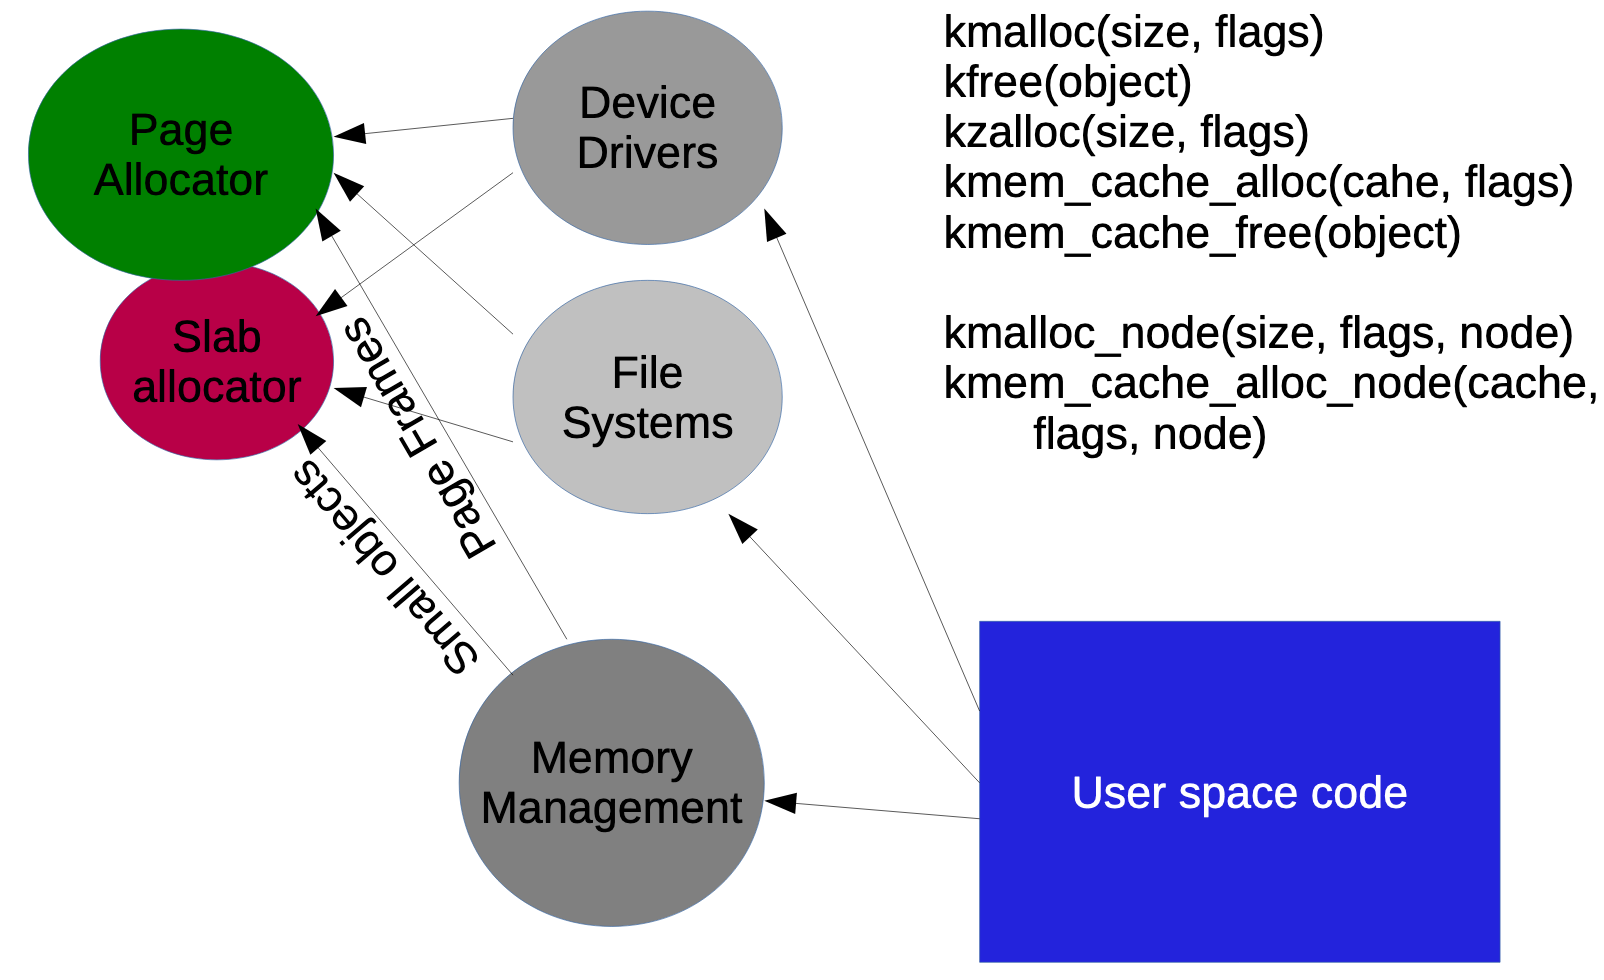
\includegraphics[width=0.7\linewidth]{system-components}
%        \caption{xxxx}
    \end{figure}

    ref: \href{https://events.static.linuxfound.org/sites/events/files/slides/slaballocators.pdf}{slaballocators.pdf}

\end{frame}
%------------------------------------------------
\begin{frame}[plain,t]    
    \frametitle{SLAB分配器}

    SLAB分配器源于 Solaris 2.4 的分配算法,工作于内存物理页分配算法之上,管理特定大小对象的缓存,进行快速高效的物理内存分配。\pause
    \begin{columns}
        \begin{column}{0.5\textwidth}
          \begin{itemize}
              \item 想解决的问题
              \begin{itemize}
                  \item 内核对象远小于页的大小
                  \item 内核对象会被频繁的申请和释放
                  \item 内核对象初始化时间超过分配和释放内存总时间
              \end{itemize}
          \end{itemize}
        \end{column} \pause
        \begin{column}{0.5\textwidth}
          \begin{figure}
              \centering
              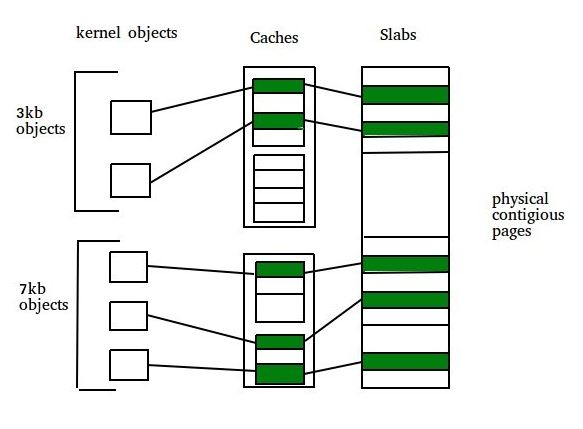
\includegraphics[width=1.0\linewidth]{Slab-Allocation}
      %        \caption{xxxx}
          \end{figure}
        \end{column}
    \end{columns}
\end{frame}
%------------------------------------------------
\subsection{SLAB} % A subsection can be created just before a set of slides with a common theme to further break down your presentation into chunks
%------------------------------------------------
\begin{frame}[plain,t]    
    \frametitle{SLAB分配器的特征}
    \begin{itemize}
        \item 为每种使用的内核对象建立单独的缓冲区
        \item 按对象大小分组
        \item 两种SLAB对象状态:已分配或空闲
        \item 三类缓冲区队列:Full、Partial、Empty
        \item 优先从Partial队列中分配对象
        \item 缓冲区为每个处理器维护一个本地缓存
    \end{itemize}
\end{frame}
%------------------------------------------------
\begin{frame}[plain,t]    
    \frametitle{SLAB分配器的结构}
    \begin{figure}
        \centering
        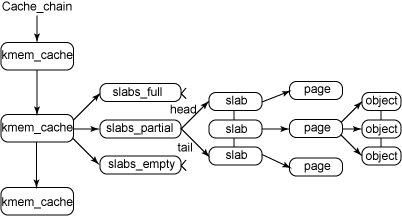
\includegraphics[width=0.9\linewidth]{slab-structure}
%        \caption{xxxx}
    \end{figure}
\end{frame}
%------------------------------------------------
\begin{frame}[plain,t]    
    \frametitle{CPU缓存着色与SLAB}
    \begin{figure}
        \centering
        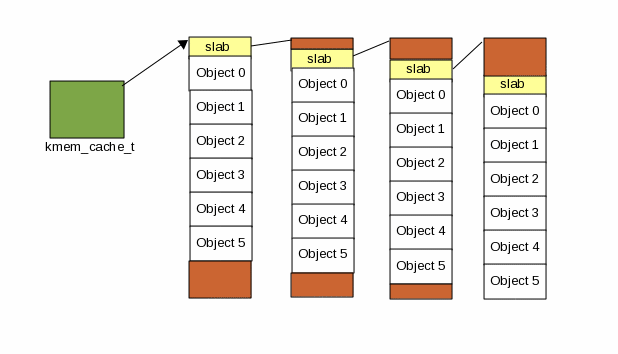
\includegraphics[width=0.8\linewidth]{slabcolor.png}
%        \caption{xxxx}
    \end{figure}
\end{frame}
% http://www.secretmango.com/jimb/Whitepapers/slabs/slab.html
% Figure 5. Cache Coloring within slabs
%------------------------------------------------
\begin{frame}[plain,t]    
    \frametitle{SLAB的数据结构}
    \begin{figure}
        \centering
        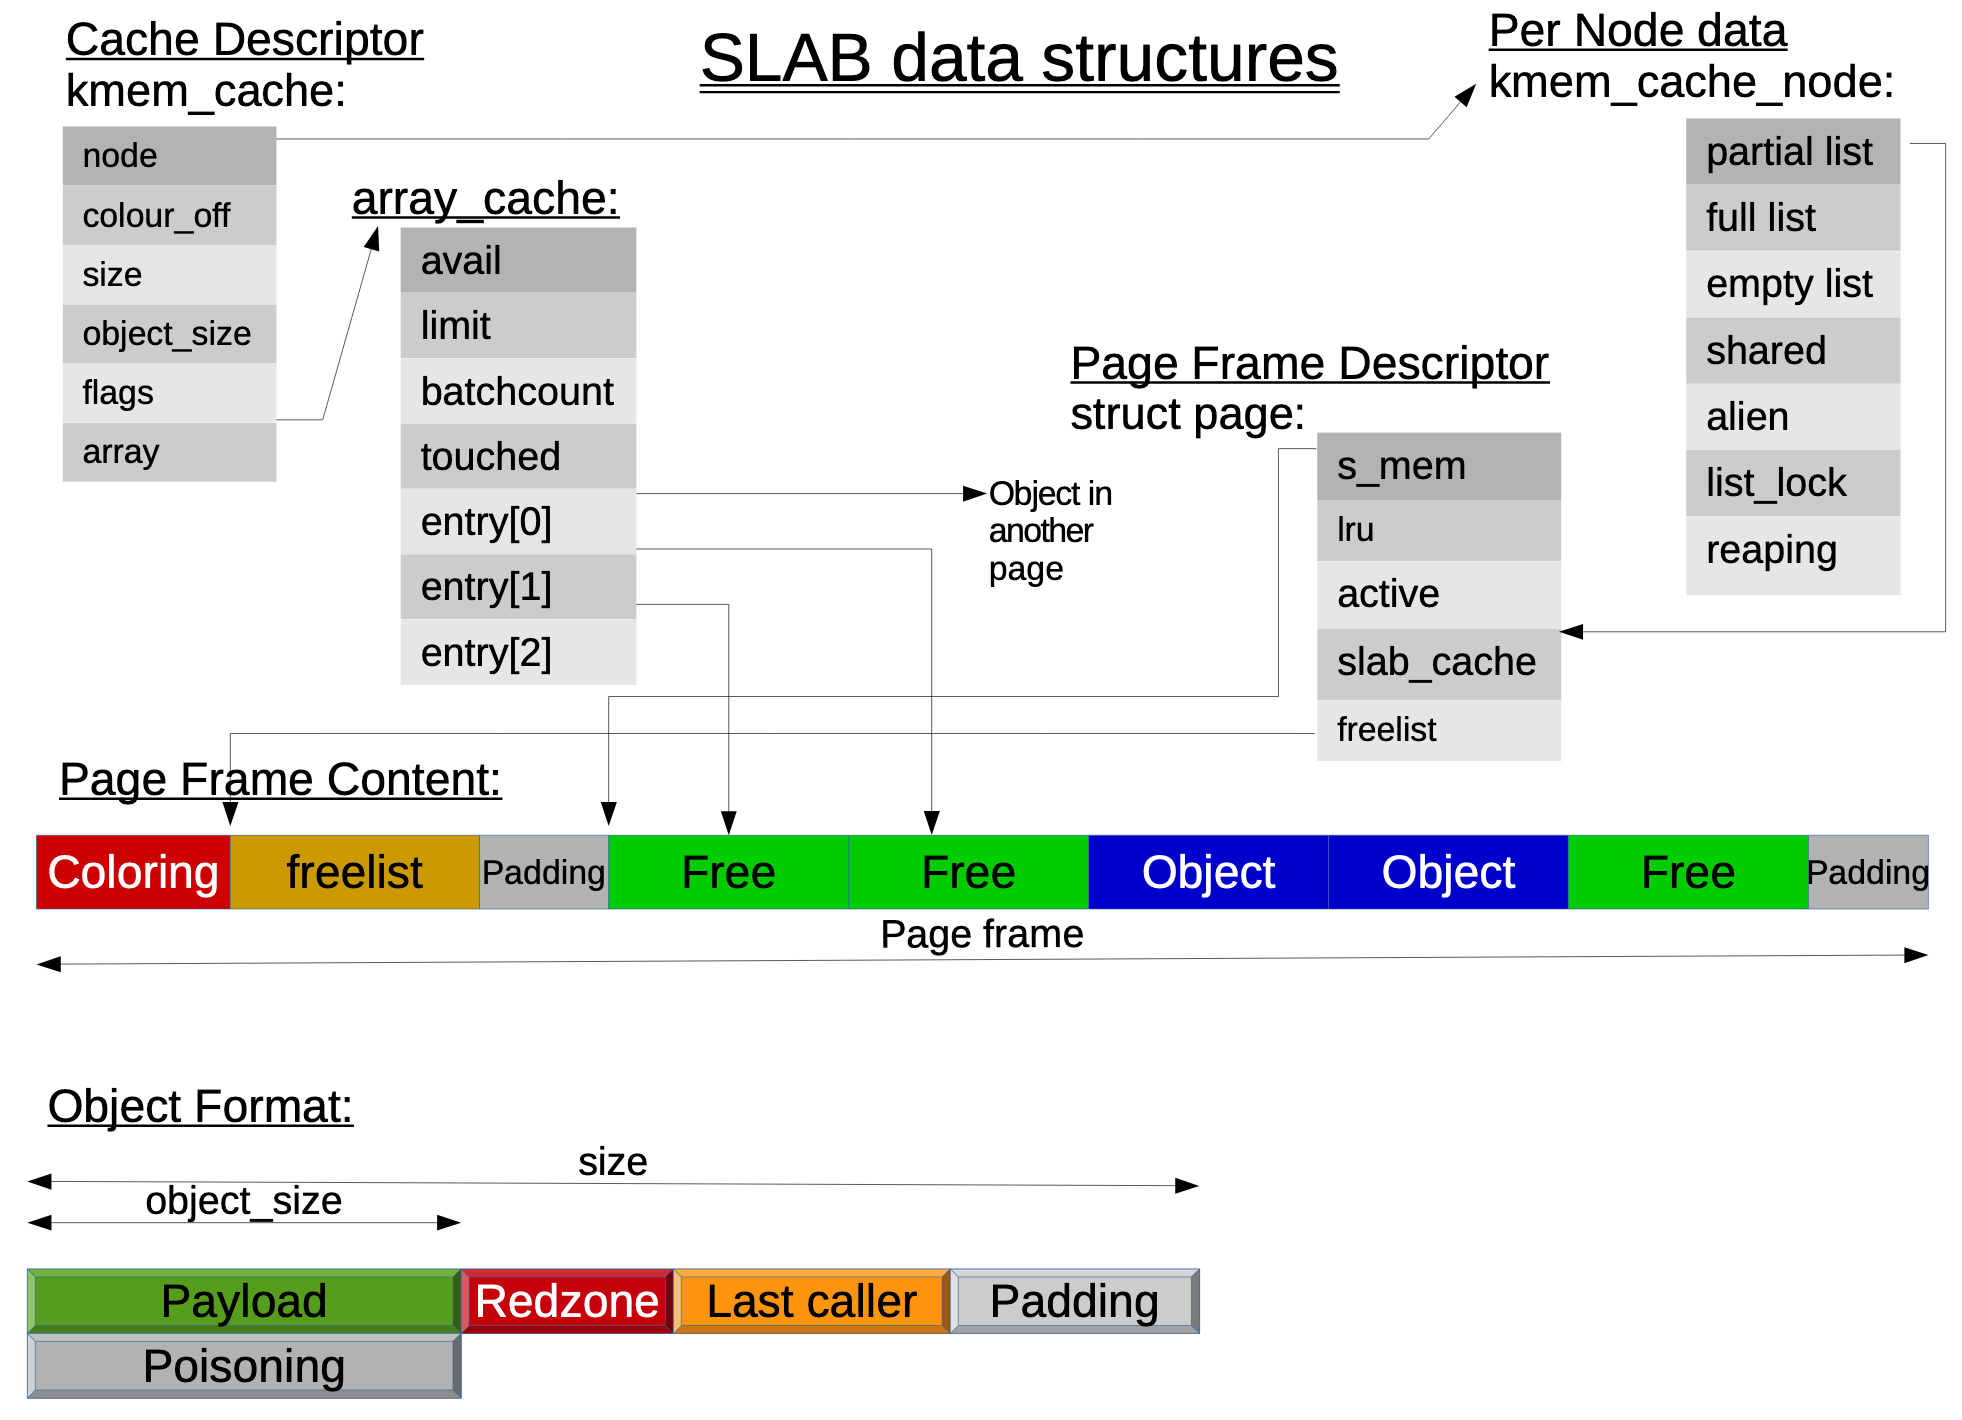
\includegraphics[width=0.65\linewidth]{slab}
%        \caption{xxxx}
    \end{figure}
\end{frame}
%------------------------------------------------
\begin{frame}[plain,t]    
    \frametitle{单个SLAB分配器结构}
    \begin{figure}
        \centering
        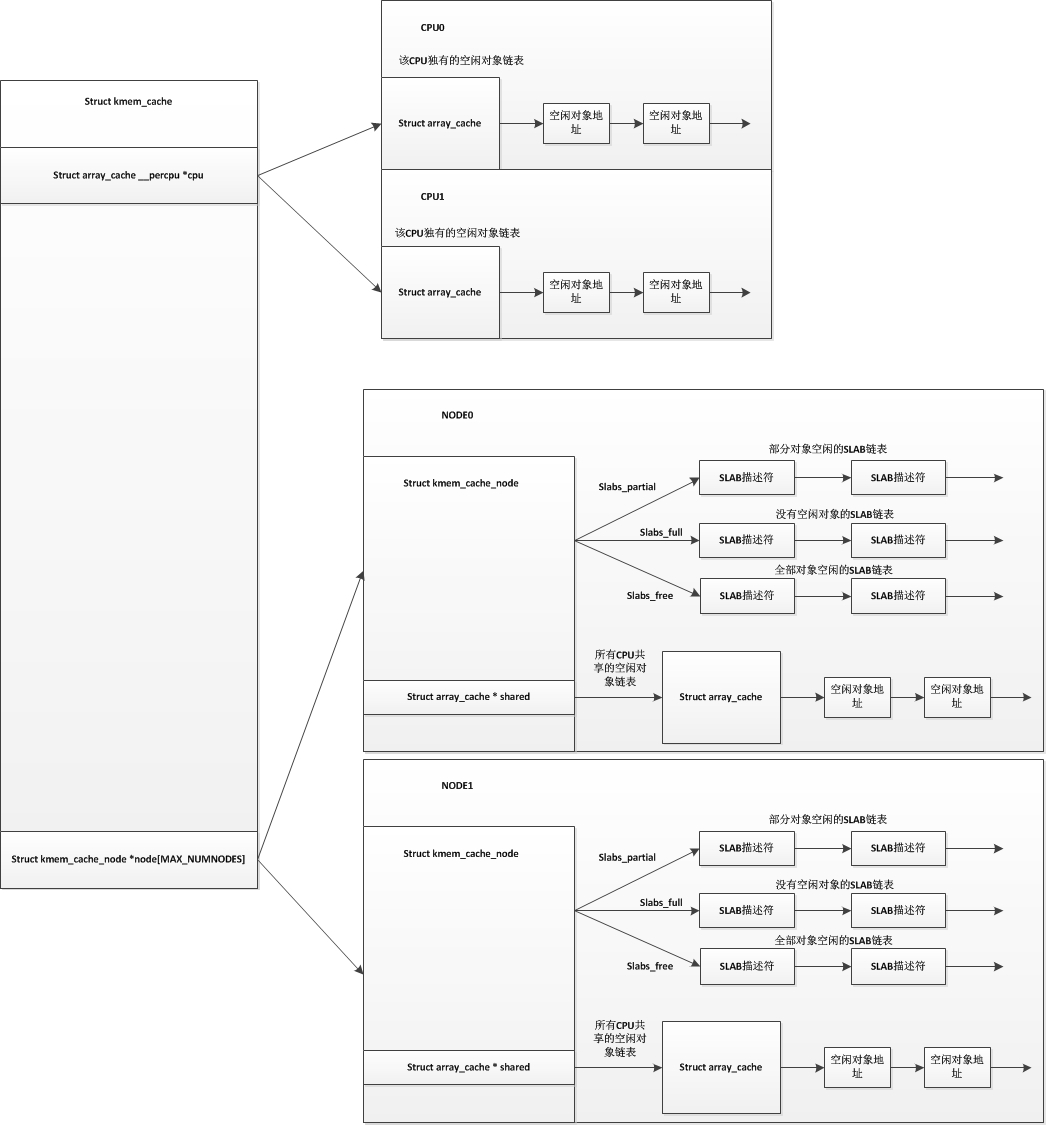
\includegraphics[width=0.45\linewidth]{single-slab}
%        \caption{xxxx}
    \end{figure}
\end{frame}
%------------------------------------------------
\subsection{SLOB} % A subsection can be created just before a set of slides with a common theme to further break down your presentation into chunks
%------------------------------------------------
\begin{frame}[plain,t]    
    \frametitle{SLOB分配器}
    \begin{itemize}
        \item SLOB分配器是针对嵌入式系统的SLAB简化版本
        \begin{itemize}
            \item 没有本地CPU高速缓存和本地节点的概念
            \item 只存在三个全局partial free链表
            \item 链表按对象大小来划分
        \end{itemize}
    \end{itemize}
\end{frame}
%------------------------------------------------
\begin{frame}[plain,t]    
    \frametitle{SLOB分配器的数据结构}
    \begin{figure}
        \centering
        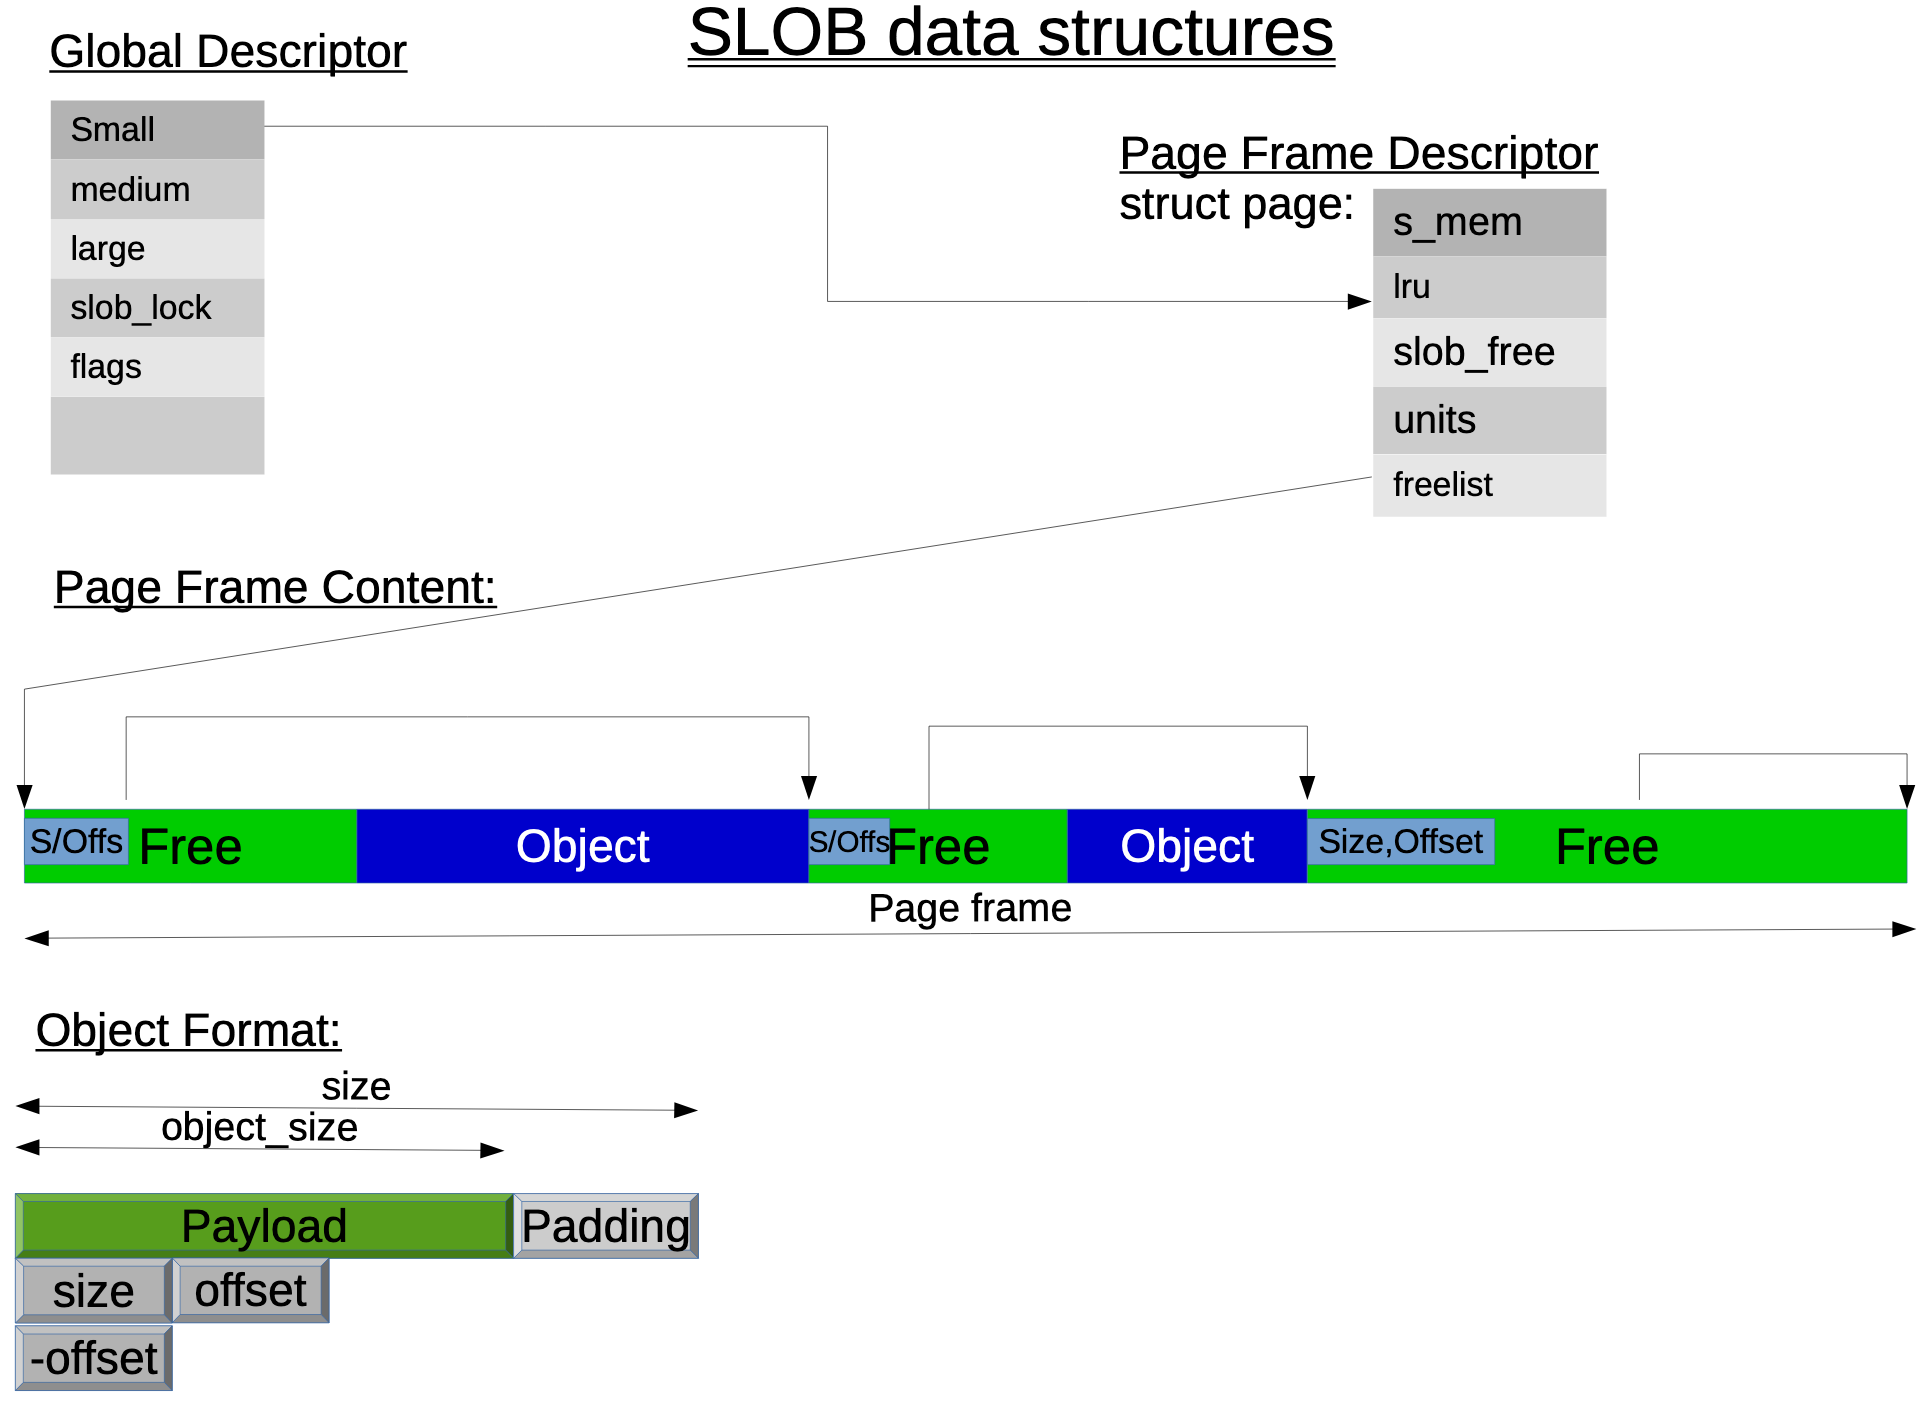
\includegraphics[width=0.65\linewidth]{slob}
%        \caption{xxxx}
    \end{figure}

\end{frame}
%------------------------------------------------
\subsection{SLUB} % A subsection can be created just before a set of slides with a common theme to further break down your presentation into chunks
%------------------------------------------------
\begin{frame}[plain,t]    
    \frametitle{SLUB分配器}

    \begin{itemize}
        \item 目标

        \begin{itemize}
            \item 简化设计理念
        \end{itemize}\pause
        \item 思路

        \begin{itemize}
            \item 简化 SLAB 的结构:取消了大量的队列和相关开销
            \item 一个SLAB是一组一个或多个页面,封装了固定大小的对象,内部没有元数据
            \item 将元数据存储在页面相关的页结构
            \item 没有单独的Empty SLAB队列
        \end{itemize}
    \end{itemize}
\end{frame}
%------------------------------------------------
\begin{frame}[plain,t]    
    \frametitle{单个SLUB分配器结构}
    \begin{figure}
        \centering
        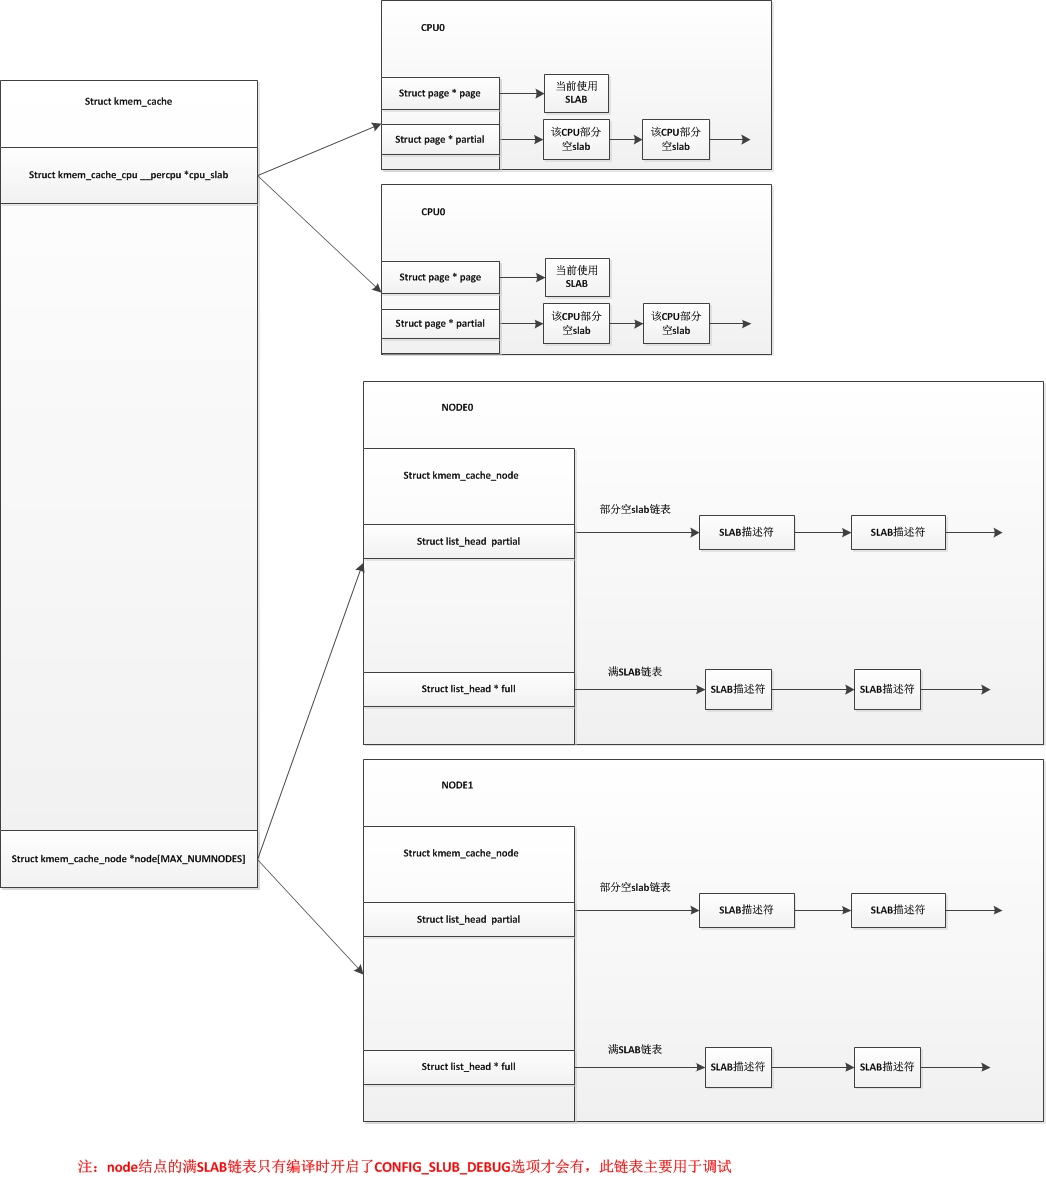
\includegraphics[width=0.4\linewidth]{single-slub}
%        \caption{xxxx}
    \end{figure}
\end{frame}
% https://www.cnblogs.com/tolimit/p/4654109.html
%------------------------------------------------
\begin{frame}[plain,t]    
    \frametitle{SLUB分配器的数据结构}
    \begin{figure}
        \centering
        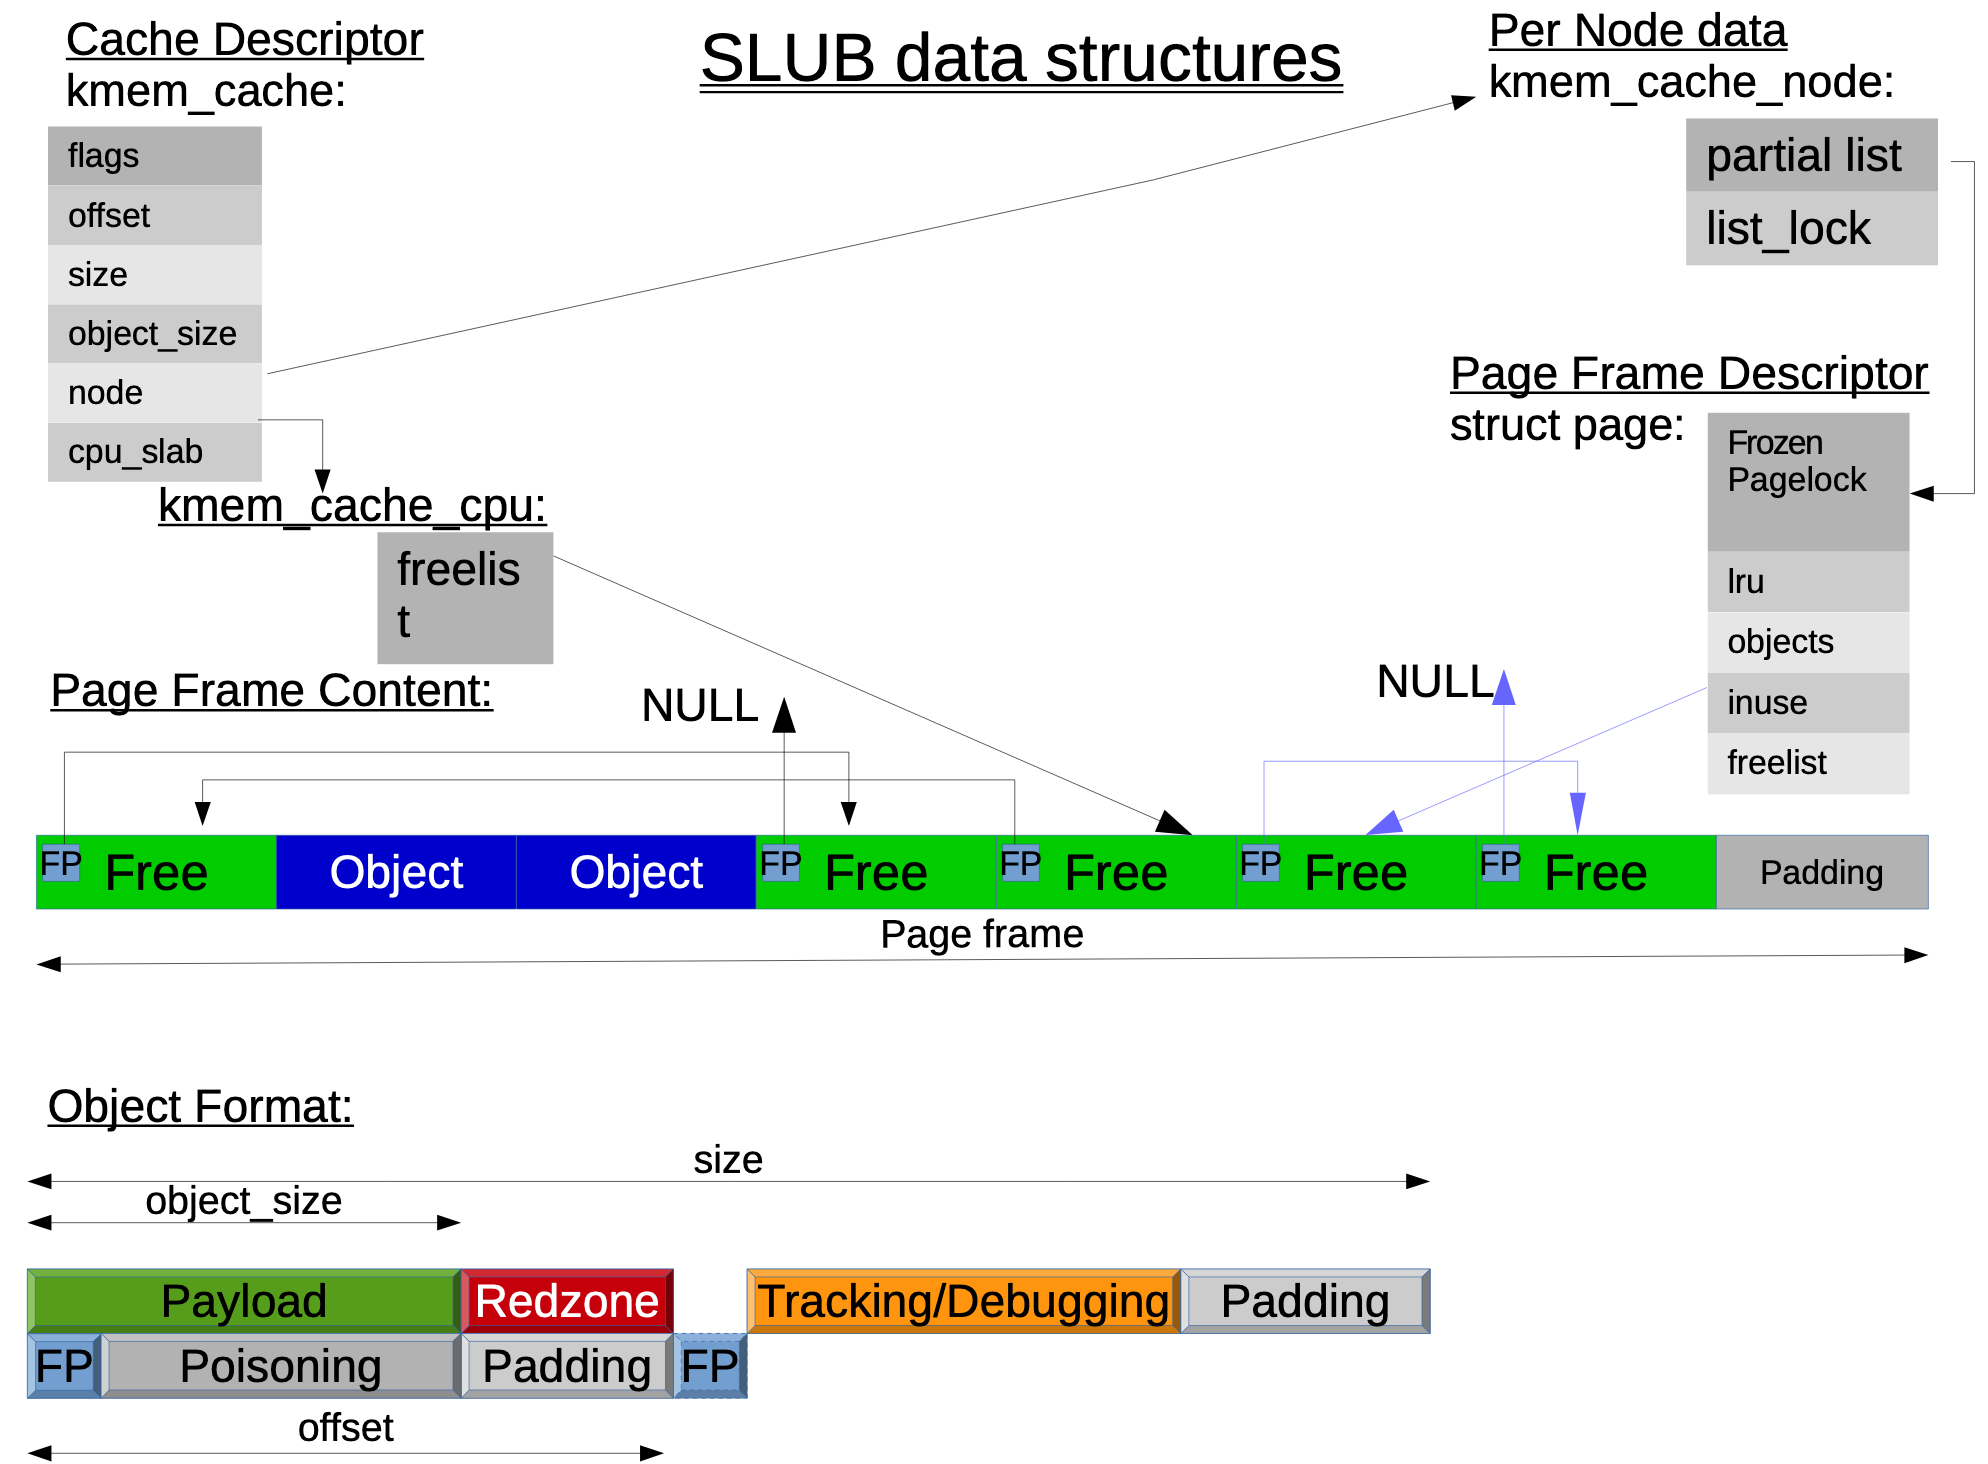
\includegraphics[width=0.65\linewidth]{slub}
%        \caption{xxxx}
    \end{figure}
\end{frame}
%----------------------------------------------------------------------------------------

\end{document}
